\chapter{Introduction}
\label{chapter:introduction}

\section{Robots in Human Environments}

The vision promised by Karel \v{C}apek in his 1921 science fiction play R.U.R, in which the word \textit{``robot"} was used the first time, featured intelligent autonomous systems that co-existed and worked for humans. The reality almost a century later today is that robots do exist, however almost all of them operate in factories, physically separated from human workers. With this separation, the safety of humans is ensured. However, it is now becoming clear that robots can provide much more value if they operate in human environments, assisting people in daily tasks. With the recent improvements in hardware and software systems and in robotics research, development of such robots is not science fiction anymore. According to International Federation of Robotics (IFR), $ \$2.2$ billion worth of personal robots were sold in the year 2014, including robotics vacuum cleaners, lawn mowers, educational and entertainment robots. This disruptive technology will make fascinating new applications possible, in contexts such as homes, hospitals, offices and factories, including but not limited to: delivery, elderly care, collaborating on an assembly line and household tasks such as cleaning. The feasibility and reliability of such applications will determine their business value, while potentially generating a new industry. Therefore, any development in this field is a step toward realization of \textit{intelligent} and \textit{social} robots.

\section{Robots that Navigate in Human Environments}

The most important difference of a robot from a computer is actuation: the ability to move in the physical world. Perhaps the most fundamental capability for a mobile robot is \textit{navigation} from one location to another. Advances in mapping, localization and path planning research in the past decades made indoor navigation a common capability for mobile robots. 

Robots occupy the same physical space with us, therefore should be aware of the fact that their movements would be observed and reacted by humans. As we start having more and more mobile robots in human environments, we will notice that robots can move in a way that is not socially acceptable by people. For example, robots can cut people's paths, navigate uncomfortably close to people and move in a way that doesn't signal where it is intended to go. Investigating the context of robots in human environments gave rise to the sub-field of robotics: Human-Robot Interaction (HRI). This relatively new research field extends in many directions with a common goal: robots that will perceive its environment, reason and act in a safe way to facilitate people's lives. Thus, a robot that will serve to people should not only be a machine, but also respect social rules and protocols.

\section{The Science of Personal Spaces}
\label{sec:personal_spaces}

How should mobile agents adjust their spatial relationships with respect to humans? In fact, humans already have a framework for this problem. It is called the \textit{proxemics}, coined by Hall \cite{hall1966hidden}, which studies of our use of space and the spatial separation individuals naturally maintain. One of Hall's main findings is that humans adjust the amount of distance between them in four distance levels: intimate, personal, social and public distances, depending on the intimacy level between individuals. Another important research work in human-human is Kendon's F Formations \cite{kendon1990conducting}, which studies the formations people tend to take in groups settings.

Personal spaces are influenced by other factors such as cultures, the range of their sensory systems, and postures of the two actors. Although it is not known whether it is best to model robot navigation behaviors after humans, applying the concepts from human-human spatial studies is a good start. This is especially true given that non-expert users today never interacted with a mobile robot and thus are likely expect the robot to behave within human social norms.

\section{Semantic Maps}
\label{sec:semantic_maps}

Robots keep a representation of its environment to enable navigation behaviors, and this representation is usually in the form of a discrete metric \textit{map}, where each grid cells represent whether that position is occupied with an obstacle or not. Mobile robots that use such a map can accept navigation goals in metric coordinates (i.e. go to coordinate (5.2, -1.3)), however exact coordinates may not be the most intuitive way to communicate goals for human users. Robots that navigate in human environments will need to accept human-friendly navigation goals. A map for such robots should facilitate establishment of a \textit{common ground} between the robot and its user and enable referencing to the same spatial elements. For example, the robot should be able to understand commands such as ``go to the kitchen table" or ``wait outside Joe's room". This is only possible with a richer map representation that includes \textit{semantic} information. In particular, if the humans and robots need to communicate over navigation goals that involve objects, landmarks or rooms, a map should include information about these.

\section{Tour Scenario}
\label{sec:tour_scenario}

One method to familiarize the robot to a new human environment is the \textit{Tour Scenario} \cite{topp2008human}, by which the robot interactively collects semantic information. Here is how the Tour Scenario is defined: After the robot product is shipped and unpacked in a home or office setting, a human user takes the robot on a tour so the robot can create a representation of the environment. In this interactive scenario, the robot learns basic information about the surroundings, while following the user. During the tour, the user can point out and identify relevant places and objects which the robot can utilize for future tasks. It is likely that the a commercial robot product that has the capability of the familiarizing task will include both human-interactive and automatic components (i.e. automatic object recognition). In this thesis we focus on the interactive components.



\section{Challenges}

There are four primary challenges in developing a practical robotic system that navigates using semantic information. From the robot's perspective, the interesting research questions are:

\begin{itemize}
\item Where are the people?
\item How should I move around humans?
\item How can I acquire semantic information about this environment?
\item How can I utilize this semantic information to improve navigation?
\end{itemize}

The challenges laid out by these questions will be addressed for the remainder of this section, and the answers will be discussed throughout this thesis.

\subsection{Robust People Tracking}

In order to be engaged in any kind of meaningful spatial interaction with humans, a robot has to be able to track people around it. Robust tracking of people is necessary to ensure high success rates for HRI tasks.

We use a tracking system that estimates the positions and velocities of humans, using three distinct body part detectors. These detectors are the leg detector, torso detector and upper body detector. Use of multiple modalities is leveraged to increase the robustness of tracking and provide more coverage around the robot. The detections are consolidated into position estimations using a Kalman Filter.

\subsection{Social Navigation}

Path planing for mobile robots has traditionally been considered a shortest-path problem. While this leads to sound solutions and collision-free paths, the behavior of the robot may be perceived as unsafe or unnatural by human observers. When a robot is navigating in an human environment, the most important consideration is the safety of people. Moreover, even if a robot's motions are safe, they can still cause discomfort. For example, sudden appearance of a robot can bother people or cutting in between two people while they are in a conversation may be considered rude behavior. Therefore, social factors should also be taken account along with effectiveness of robot motions. Borrowing the idea from Sisbot \cite{sisbot2007human}, we attach personal spaces and social constraints as costs to map cells while planning a path. Our planner also takes into account people's reaction to the robot's motion. Humans routinely use anticipation during navigation. For example, in a hallway encounter, one person may lean towards the left of the corridor, expecting the other to take right. We aim to give this anticipation ability to robots. Furthermore, we develop interactive navigation applications where the task of the robot is to follow a person or to a guide a person to a location.

\subsection{Interactive Map Annotation}

The question of how semantic maps could be useful for various tasks is addressed in Section \ref{sec:semantic_maps}. People may want to provide custom labels to landmarks, objects and waypoints instead of generic ones. By using unique labels, ambiguities can be resolved. For example, if an automatic object recognizer is utilized, the robot could be confused if it is given the command ``bring my laptop" and there are multiple laptops in the environment. Moreover, the ability to label objects and locations would complement automatic recognizers. For example, if an object recognition system makes an error, a user would be able to change the object's label. Our solution to annotate maps is to maintain a common ground between a human and and the robot is via the Tour Scenario, as described in Section \ref{sec:tour_scenario}.

\subsection{Situation Awareness for Navigation}

Metric maps provide a single type of information: whether a grid cell is occupied with an obstacle or not. While this kind of a simplistic map representation may be sufficient for some navigation tasks, if the robot needs to communicate with human users about its goals, it should have a richer map representation of the environment. The robot can leverage the semantic information presented in the map and increase its usefulness for navigation tasks.

%None of the works in this field leverage the semantic maps to increase situational awareness.

Simply put, Situation Awareness is knowing what is going on around you. It can be achieved in various contexts for robot navigation. Person following with a robot is a widely studied research topic, however in the literature it is not usually considered \textit{why} the robot is following the person and how the task context can be used to increase effectiveness. For example, during the Tour Scenario, the robot may employ a more intelligent following strategy if it knows the user will be pointing at landmarks and places. Furthermore, consider handling of the doors while following. If the robot does not know that it is standing on a doorway, it can block the path for others. If the door is added to the semantic map, the robot can have the opportunity to handle the door passing graciously. Moreover, the robot can utilize the floor layout of the environment to adjust its speed. For example, if the robot is in a region where the chance to encounter a person is high, slowing down may be a sensible action to take.


%For example, when the robot is navigating, if the robot knows that it is in a region of high human density, slowing down may be a sensible action to take.



%Goal Points
%Door, landmarks, objects as special cases.
%Safety: Use map layout for speed adjustments, speed up

\section{Scope and Context}

In this section, we provide an overview of the assumptions of our research.  At a high level, autonomous robots perceive its environment, reason the situation, act in the world. In the HRI context, the research in perception is focused on improving the robot's ability to ``see" its environment, identify objects and humans. The reasoning part is focused on deciding on ``what to do" and ``how to do" in a given situation. Acting part is focused on the execution and control of motions, as well as the design of mechanisms. This thesis mainly focuses on the reasoning part while also offering a solution to the perception part.

We assume that we have a wheeled mobile robot platform. Even though some of our algorithms are derived for a non-holonomic robot with differential drive actuation, it is a technical limitation rather than a conceptual one, as they can be applied to mobile robots with different mechanisms with minor changes. We further assume that the robot is self-contained: equipped with on-board sensors, is capable of creating a map of the environment with an existing Simultaneous Localization and Mapping (SLAM) package, and then able to localize itself in this created map as it moves in the environment.

Furthermore, we focus on scenarios where people in the environment are standing or walking, because that's the most common body pose the robot would encounter. 

A user can control the robot via tablet or smartphone apps. Similar functionality could be achieved with a speech dialog system, however we chose touch-based interfaces due to their ubiquity and reliability.

\section{Thesis Overview}
\subsection{Thesis Statement}

%Non-expert users can label objects, landmarks and locations while giving a tour to a mobile robot, where the labeled entities enable situational awareness and serve as end goals, which robots can navigate to, by taking into account the personal spaces of nearby humans and social factors.

Non-expert users can effortlessly interact with and control a mobile robot through the use of semantic maps and spatial rules of engagement.

\subsection{Contributions}

\begin{itemize}
%\item Development of a multimodal person detection and tracking system using on-board sensing, with a particular focus on 360$^{\circ}$ coverage
\item A method for a human to take a mobile robot on a tour and interactively add labeled objects, landmarks and locations to the robot's map using natural deictic gestures and later use these labeled entities as end goals for navigation
\item Development of a navigation planner that takes into account social factors, and people's reactions to robot's motions
\item Development of a person guidance behavior and its application to indoor wayfinding for blind users
\item Development of a person following behavior and its usage for telepresence robots
\item Demonstration of situation awareness for person following behavior, targeted at the Tour scenario
\end{itemize}


\subsection{Document Outline}

The structure of this thesis is shown in Figure \ref{fig:thesis_outline}.

\begin{figure}[ht!]
\centering
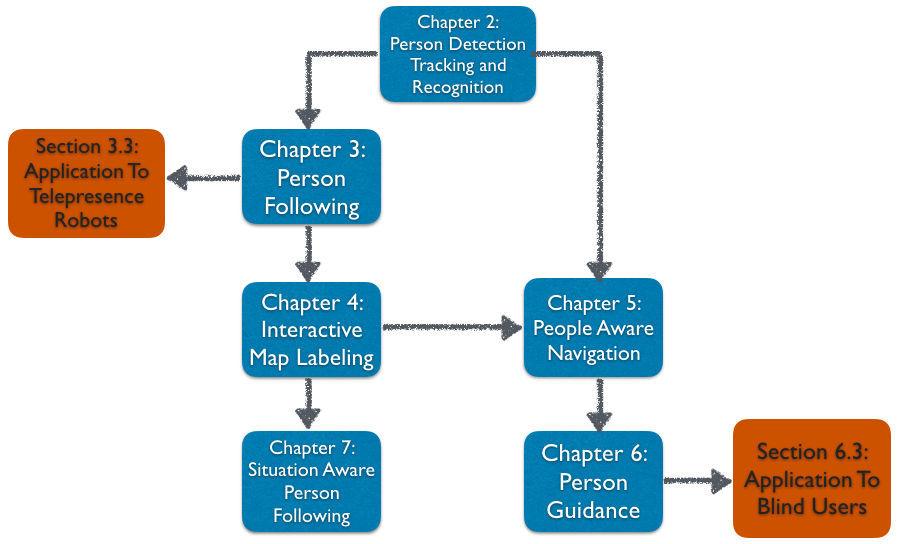
\includegraphics[width=1.0\textwidth]{pics/outline_new}
\caption{Thesis Outline}
\label{fig:thesis_outline}
\end{figure}

The first prerequisite for a socially aware robot is detecting and tracking people. \textbf{Chapter \ref{chapter:multimodal_person_detection_and_tracking}- Person Detection, Tracking and Recognition} presents our method of leg detection, torso detection and face recognition and how the robot estimates the positions of nearby people using these detections.

When a robot is able to keep track of the positions of nearby people, it can follow a user. \textbf{Chapter \ref{chapter:person_following} - Person Following} describes how the robot follows a person. Additionally, an application of person following for telepresence robots is presented in Section \ref{sec:following_application_to_telepresence}.

If a robot has the capability to follow a person, a user can take the robot on a tour around the house and teach landmarks to the robot. \textbf{Chapter \ref{chapter:map_annotation} - Interactive Map Labeling} describes our semantic map representation, the process of interactively labeling landmarks, the user interface and how to detect pointing gesture targets.

The ability to track nearby people also gives the robot the capability to conduct socially aware navigation toward labeled landmarks. \textbf{Chapter \ref{chapter:navigation_among_people} - People-Aware Navigation} discusses how we extract goal points from semantic maps, and a people-aware planner for navigating from a start position to a goal position.

If a robot is able to navigate toward a goal position or a landmark, it can also guide people to the same goals. \textbf{Chapter \ref{chapter:person_guidance} - Person Guidance} presents the behavior design of a tour guide robot and how the robot can guide a person to a goal. Furthermore, we present an application of person guidance for visually impaired users in Section \ref{sec:guidance_blind_users}.

The person tracking and following capability, combined with the existence of labeled landmarks, enables the robot to react to social situations during following. \textbf{Chapter \ref{chapter:following_situation_aware} - Situation Aware Person Following} discusses some problematic scenarios that could be encountered during following and presents our design of robot behaviors for these situations.

\textbf{Chapter \ref{chapter:conclusion} - Conclusion and Discussion} discusses the contributions of this thesis, lessons learned during the research program and future work in this area of research.

\textbf{Appendix \ref{chapter:telepresence_user_study_survey_questions}} lists telepresence user study survey questions.

\textbf{Appendix \ref{chapter:vibration_pattern_analysis_for_haptic_belts}} gives details of the user study on haptic belts for guiding blind people.
